This section introduces the OD-conditioned generation task, the compared model families, and the physics-informed residual formulation.

\subsection{Problem Setup}
Trajectories are represented in a grid coordinate system. Let $\mathbf{p}_t \in \mathbb{R}^2$ denote the 2D position at step $t$ (grid indices in $[y,x]$ order), and define step displacement (velocity) as
\begin{equation}
  \mathbf{v}_t = \mathbf{p}_{t+1} - \mathbf{p}_t .
  \label{eq:vel_def}
\end{equation}
With dt-fixed sampling, $\mathbf{v}_t$ has explicit temporal meaning.
We denote the observed history as $\mathbf{X}=\{(\mathbf{p}_t,\mathbf{v}_t)\}_{t=-H+1}^{0}$ and the future velocities as $\mathbf{Y}=\{\mathbf{v}_t\}_{t=1}^{F}$.
Given a global context vector $\mathbf{c}$ (time features and OD endpoints), our goal is to model the conditional distribution
\begin{equation}
  p_\theta(\mathbf{Y}\mid \mathbf{X}, \mathbf{c}).
  \label{eq:cond_dist}
\end{equation}

\subsection{Model Framework}
We compare a deterministic regression baseline, conditional diffusion generators, and our residual formulation that explicitly separates macroscopic scale from stochastic variability (Figure~\ref{fig:method-overview}).

\begin{figure}[t]
  \centering
  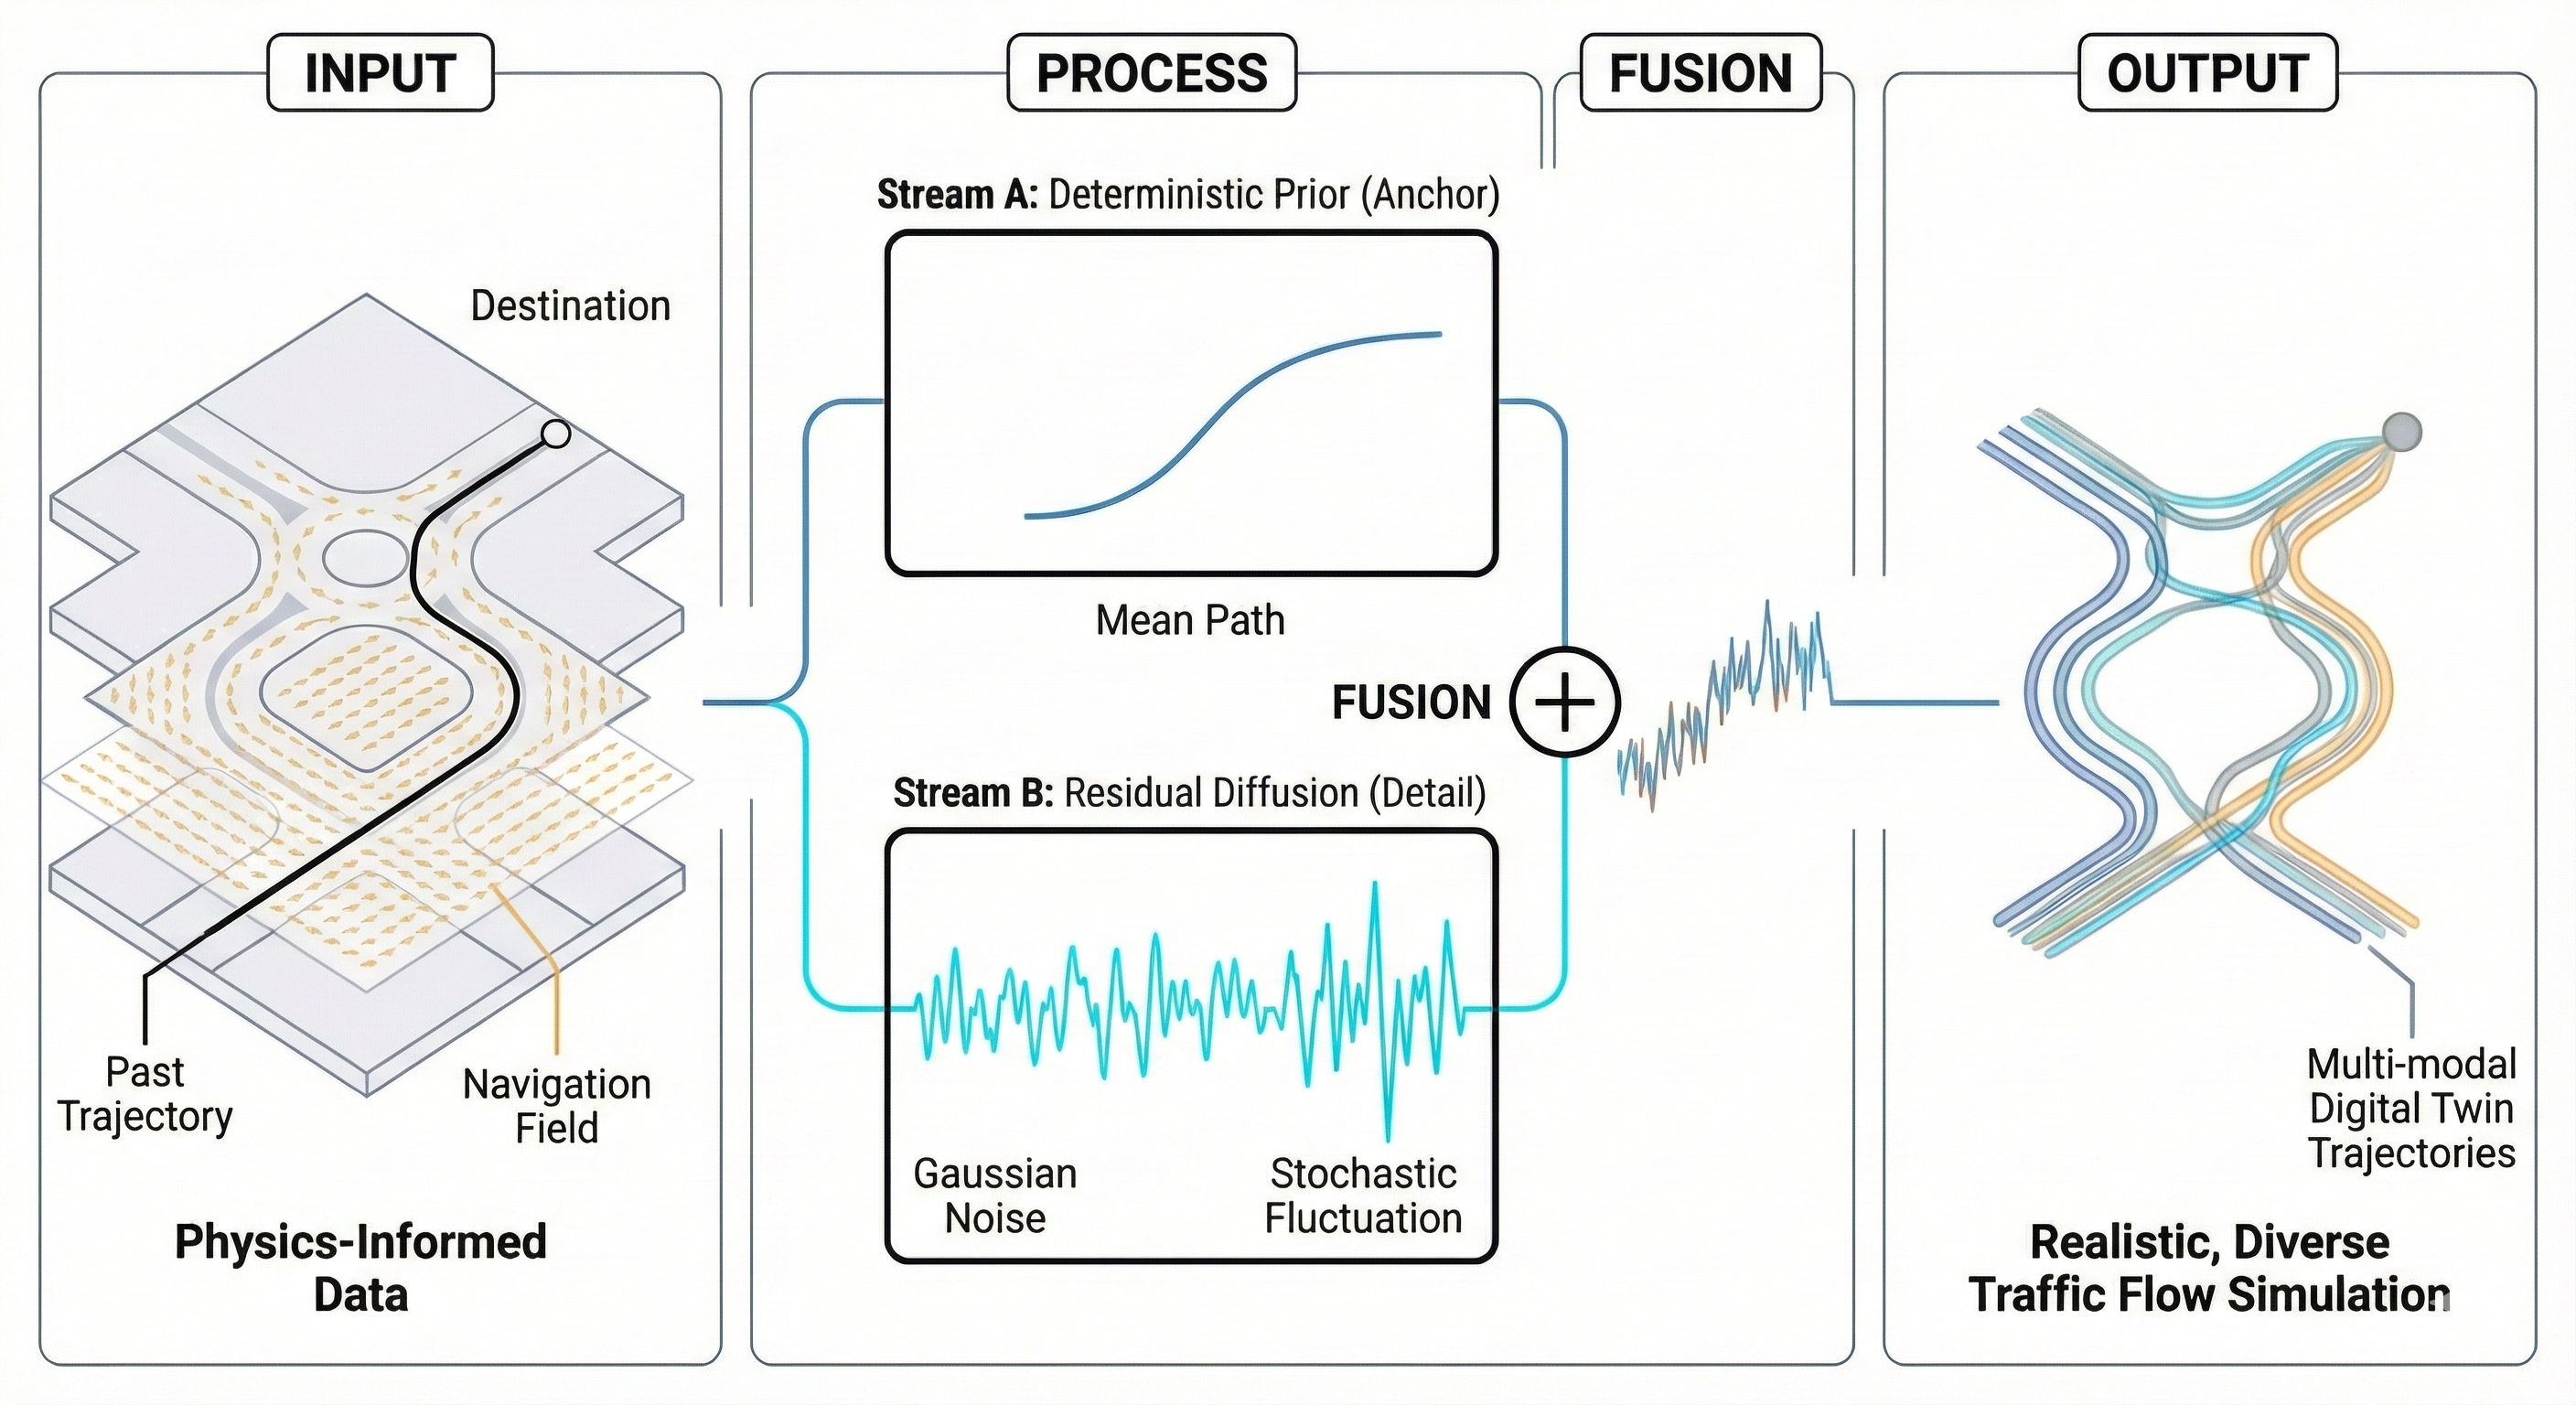
\includegraphics[width=0.95\linewidth]{figures/fig1_framework.png}
  \caption{Framework overview. A frozen deterministic prior (anchor) captures low-frequency OD-driven motion. A diffusion model samples high-frequency residuals (detail), optionally conditioned on a train-only navigation-field prior. The sum yields diverse trajectories while preserving macroscopic motion statistics.}
  \label{fig:method-overview}
\end{figure}

\paragraph{Deterministic baseline (L2 regression).}
The baseline predicts a single future velocity sequence by minimizing L2 error (equivalently $K=1$ at inference).

\paragraph{Conditional diffusion generator.}
We adopt a denoising diffusion probabilistic model (DDPM) \citep{ho2020ddpm} to sample future velocity sequences conditioned on $(\mathbf{X},\mathbf{c})$. The model is trained to predict diffusion noise with the standard objective
\begin{equation}
  \mathcal{L}_{\mathrm{diff}} =
  \mathbb{E}_{\mathbf{y}_0,t,\epsilon}\left[\left\|\epsilon - \epsilon_\theta(\mathbf{y}_t,t,\mathbf{c})\right\|_2^2\right],
  \label{eq:ddpm_loss}
\end{equation}
where $\mathbf{y}_0$ is the clean future velocity matrix, $\mathbf{y}_t$ is its noisy version at timestep $t$, and $\epsilon \sim \mathcal{N}(\mathbf{0},\mathbf{I})$.

\paragraph{Physics conditioning via a train-only navigation field.}
To inject a lightweight physical prior without road-graph engineering, we construct a train-only \emph{navigation field} that summarizes local mean flow in grid space.
For each grid cell we estimate a mean displacement direction $\mathbf{u}_{ij}$ and mean speed $s_{ij}$ from the training split. At inference, we crop a local patch around the last observed position $\mathbf{p}_0$:
\begin{equation}
  \Phi(\mathbf{p}_0) \in \mathbb{R}^{3\times K\times K}, \quad
  \Phi = [\,\mathbf{u}_y,\mathbf{u}_x, s\,],
  \label{eq:nav_patch}
\end{equation}
encode it with a small CNN, and concatenate the resulting embedding with the global condition.

\paragraph{Main method: Physics-Informed Residual Diffusion.}
Pure diffusion can exhibit \emph{macroscopic shrinkage} (under-estimated displacement and speed). We address this structurally by decomposing future motion into a deterministic prior plus a stochastic residual:
\begin{equation}
  \mathbf{v}_{1:F} = \mathbf{v}^{\mathrm{prior}}_{1:F} + \mathbf{v}^{\mathrm{res}}_{1:F},
  \qquad
  \mathbf{v}^{\mathrm{prior}}_{1:F} = f_{\mathrm{base}}(\mathbf{X}, \mathbf{c}),
  \label{eq:residual_decomp}
\end{equation}
where $f_{\mathrm{base}}$ is a frozen baseline trained under the same dt-fixed protocol. The diffusion model learns the conditional distribution of residual velocities and samples $\mathbf{v}^{\mathrm{res}}$; adding it back to the prior yields the final future trajectory.

\subsection{Evaluation Protocol}
For generative models we draw $K$ samples per condition and report both mean errors and best-of-$K$ (oracle) metrics to quantify coverage. We evaluate micro-level errors (ADE/FDE) and macro-level physical realism via mean squared displacement (MSD) curves and radius of gyration (Rog). MSD is defined as
\begin{equation}
  \mathrm{MSD}(\tau) = \left\langle \left\|\mathbf{p}_{t+\tau} - \mathbf{p}_t\right\|_2^2 \right\rangle,
  \label{eq:msd}
\end{equation}
and Rog is computed per trajectory as $\mathrm{Rog}=\sqrt{\frac{1}{F}\sum_{t=1}^{F}\|\mathbf{p}_t-\bar{\mathbf{p}}\|_2^2}$.
